\chapter{Hierarchical Physics Development}
\label{chapter: Hierarchical_Physics_Development}

Chapter 7 of the CCPP v6 Technical Documentation (\url{https://ccpp-techdoc.readthedocs.io/en/v6.0.0/}) provides an overview of the tools supported by the SCM to faciliate hierarchical systems systems development (HSD)

\section{Background}

Developing and implementing a new physics parameterization for use in an operational setting requires extensive testing and evaluation. This is to ensure that new developments aren’t yielding unexpected results and that all computational considerations are being met. From a scientific perspective, this process should be incremental and hierarchical: starting with initial testing of a simple idealized case, then progressing to fully-coupled high-resolution global forecasts on high-performance computing systems.


The CCPP-SCM provides developers working within CCPP compliant host models the ability to test their physics innovations without having to worry about the coupling to the dynamical core. This is a critical step in the model development hierarchy, providing insight on how an introduced physics change can modify the evolution of the internal physics state. However, there are still challenges, most notably the interactions between introduced changes and the other physics schemes in the suite.

\section{CCPP Suite Simulator}

\subsection{Overview}

The CCPP Suite Simulator is a CCPP compliant physics scheme that provides the ability to turn on/off physical processes in a Suite Definition File (SDF), using namelist options. This simulator `piggybacks' on an existing SDF, replacing physics tendencies with data-driven tendencies (\ref{fig:CSS_tendency_schematic}). 

\begin{figure}[h]
    \centering
    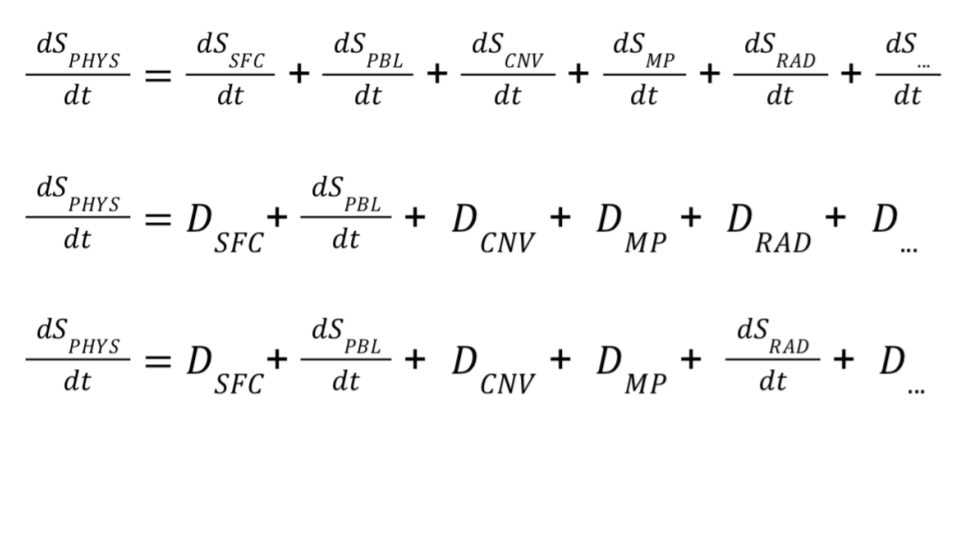
\includegraphics[width=0.80\textwidth]{images/CSS_tendency_schematic.png}
    \caption{Equation for internal physics state evolution for process-split physics suite, where S is the prognostic state and D are simulated data tendencies. Top) Standard Suite Definition File; Middle) Active PBL physics with simulated tendencies for other schemes; Bottom) Active PBL and radiation, with simulated tendencies for other schemes.}
    \label{fig:CSS_tendency_schematic}
\end{figure}

\subsection{Process-split vs. Time-split Physics Process}

Process-split physics processes are schemes that rely on the state provided the model's dynamical core, whereas time-split processes use the state provided by the previous physics process. A SDF can be any combination of time-split and process-split schemes, just as long as the appropriate interstitial schemes are created to couple the physics schemes.

\subsection{About the CCPP Suite Simulator}

The CCPP Suite Simulator (CSS) emulates the evolution of the internal physics state provided by the SDF. There are different deployments of the scheme simulator, depending on the role(s) and order of the physical processes in the SDF we are emulating (e.g. time vs. process-split), that need further attention. For instance, SDFs consisting of only process-split physics schemes can be handled simply by adding the simulator to the end of the SDF, since for process-split schemes the order is not critical to the evolution of the internal physics state. On the other hand, for SDFs that contain time-split processes, where the simulator is added is important to preserve the order of the internal state evolution.

\subsection{Enabling the CCPP Suite Simulator}

To use the CSS in the CCPP-SCM two modifications need to be made:

\begin{enumerate}
\item Add CSS, and any interstitial schemes needed for coupling the CSS to the host (e.g. SCM), to an existing CCPP SDF (or create a new SDF).
\item Modify, or create new, namelist that has the options needed to activate the CSS.
\end{enumerate}

\subsection{Namelist for the CCPP Suite Simulator}

The CSS has its own namelist, \execout{ccpp\_suite\_sim\_nml}, that needs to be added to the physics namelists used by the SCM.

\lstinputlisting[
                 basicstyle=\scriptsize\ttfamily,
                 label=lst_css_nml,
                 caption=Example namelist for CCPP Suite Simulator.
                 ]{./css_nml.txt}

\begin{itemize}
\item \execout{suite\_sim\_file}: Input file with simulated data tendencies (See \ref{section:Creating_Custom_Data_for_Simulator} for how to create input file from SCM output).
\item \execout{nprc\_sim}: Number of physical processes in the input data.
\item \execout{prc\_XYZ\_cfg}: Configuration for physical process XYZ.
\begin{itemize}
\item 0 - Active scheme; 1 - Use data
\item 0 - Process-split scheme; 1 - Time-split scheme
\item Index for scheme order (1 - \execout{nprc\_sim})
\end{itemize}
\end{itemize}

For example, in \ref{lst_css_nml}, there are two active schemes, longwave and shortwave radiaiton, and five simulated schemes: PBL, gravity-wave drag, deep/shallow convection, and cloud microphysics. The radiation, gravity-wave drag and PBL schemes are all process-split, whereas convection and cloud microphysics are time-split. 

\subsection{Creating Custom Data for Simulator}
\label{section:Creating_Custom_Data_for_Simulator}

Navigate to \execout{ccpp-scm/scm/etc/scripts/ccpp\_scheme\_sim}

Provided with the SCM are scripts to generate data for the suite simulator using output from a previous SCM run. The first script, \execout{create\_1D\_simdata.py}, extracts the physics tendencies from a user specified time interval, which are used for constant forcing in the suite simulator. The other script, \execout{create\_2D\_simdata.py}, creates a two-dimensional forcing dataset. The suite simulator interpoaltes these forcings in time.

\begin{enumerate}
\item Run the SCM, using TWPICE case with \execout{GFS\_v17\_p8} suite.
\begin{lstlisting}[language=bash]
cd ccpp-scm/scm/bin
./run_scm.py -c twpice -s SCM_GFS_v17_p8
\end{lstlisting}
\item Create 2D forcing data for the CSS, using SCM output from TWPICE case with \execout{GFS\_v17\_p8} suite.
\begin{lstlisting}[language=bash]
cd ccpp-scm/scm/etc/scripts/ccpp_scheme_sim
./create_2D_simdata.py --cases twpice --suites SCM_GFS_v17_p8
\end{lstlisting}
\item Create constant forcing data for the CSS, using SCM output, at forecast time 3600s, from TWPICE case with \execout{GFS\_v17\_p8} suite.
\begin{lstlisting}[language=bash]
cd ccpp-scm/scm/etc/scripts/ccpp_scheme_sim
./create_1D_simdata.py --cases twpice --suites SCM_GFS_v17_p8 --time 3600
\end{lstlisting}
\end{enumerate}

The data file will be written to \execout{ccpp-scm/scm/etc/scripts/ccpp\_scheme\_sim/} with the following format, \execout{data\_scheme\_sim\_DIM.CASES.SUITES.nc}.

\subsection{Example 1: Suite with Active Radiation}

\subsection{Example 2: Suite with Active Cloud Microphysics }
